%  Language: Brazilian Portuguese
\documentclass{article}
\usepackage[utf8]{inputenc}
\usepackage{graphicx}
\usepackage{natbib}


\title{Redes Neurais - CIn - UFPE}
\author{Eric Vinicius de Lima}
\date{Agosto 2021}


\begin{document}
\maketitle

\section{Introdução}

Redes Neurais é uma disciplina eletiva representada pelo código if702 ofertada no Centro de Informática. Geralmente é oferecida pelo professor Germano Vasconcelos \cite{professor} no segundo semestre de cada ano. A disciplina procura abordar o estudo de várias topologias de redes neurais e estruturas que promovem a classificação de bases de dados através do treinamento prévio. \cite{course}

\begin{figure}[h]
\centering
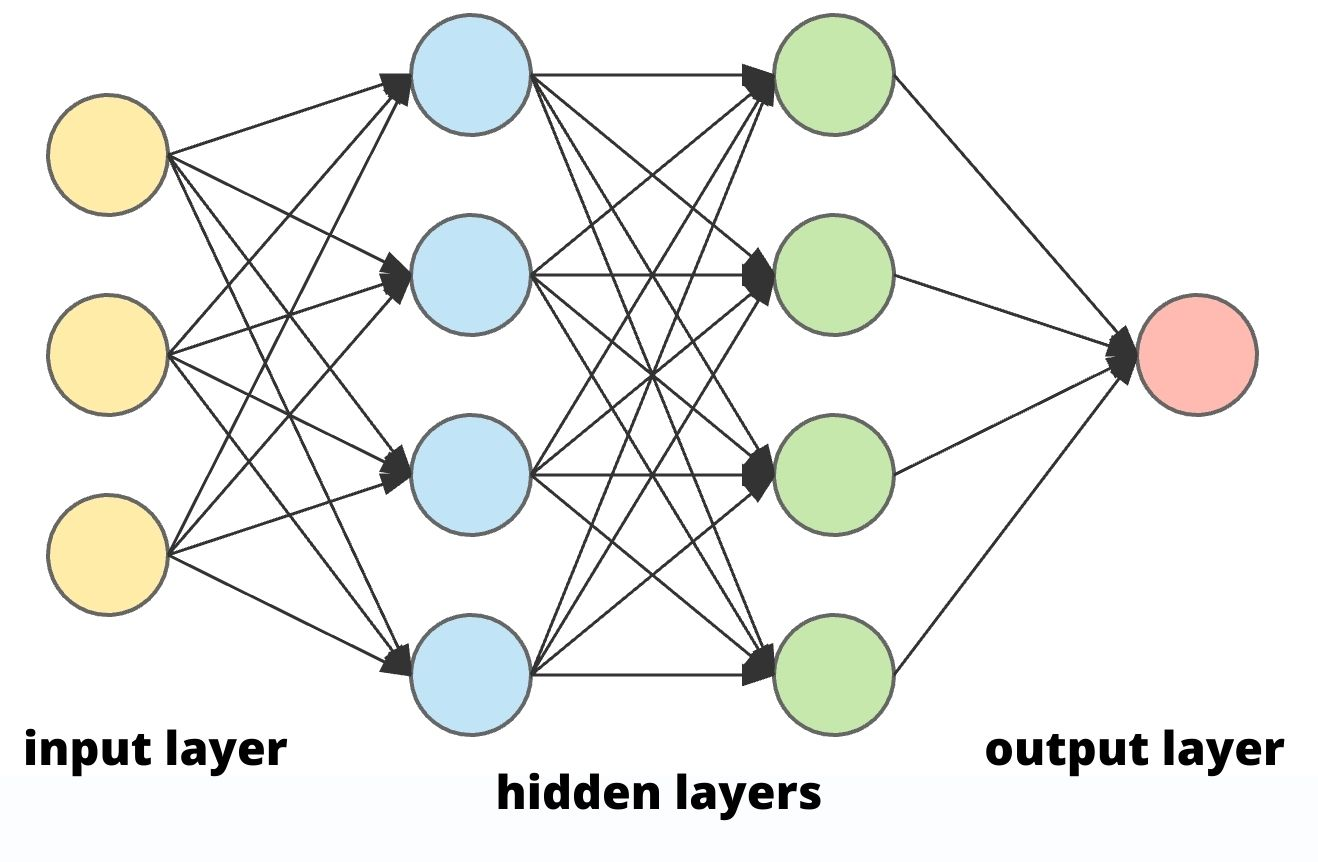
\includegraphics[scale=0.2]{layers.jpg}
\caption{Camadas em uma Rede Neural \citep{figure1}}
\label{figura_1}
\end{figure}

O curso aborda os seguintes temas \cite{course}:
\begin{itemize}
    \item Fundamentais (matemáticos e de aprendizagem) \item Arquiteturas e Modelos Redes feedforward (Adaline e Perceptrons, MLP, RBF e SVM) 
    \item Redes recorrentes (Rede de Jordan e Elman) \item Redes auto-organizáveis (modelos de ART, de Kohonen e de Hopfield).
\end{itemize}


\section{Relevância}

As redes neurais também são idealmente desenvolvidas para ajudar as pessoas a resolver problemas complexos em diversas situações da vida real. Elas podem aprender e modelar relações entre entradas e saídas de dados que são não-lineares e complexos; realizar generalizações e inferências; revelar relacionamentos, padrões e predições ocultas e modelar dados altamente voláteis (como dados de séries temporais financeiras) e variâncias necessárias para prever eventos raros (como detecção de fraudes) . \citep{importance}

\begin{figure}[h]
\centering
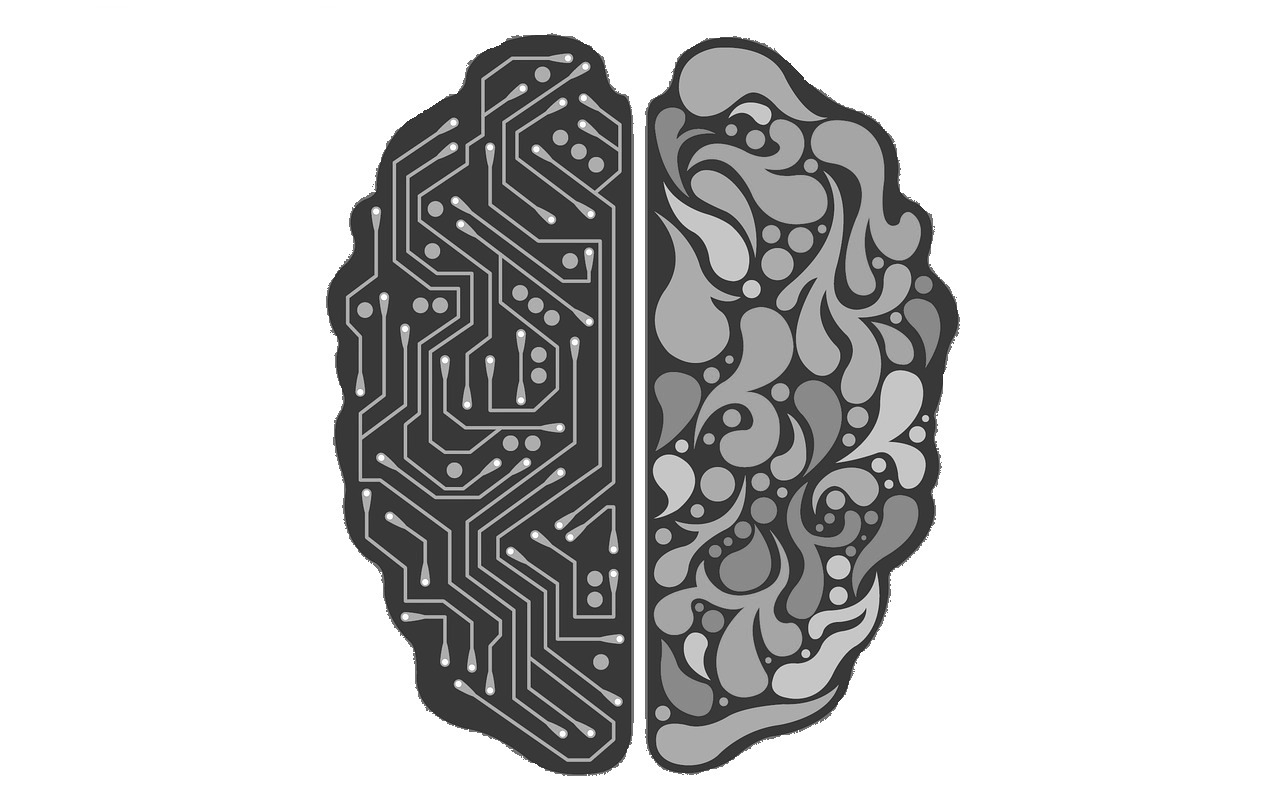
\includegraphics[scale=0.2]{brain}
\caption{Redes Neurais artificiais e biológicas\citep{figure2}}
\label{figura_2}
\end{figure}

Como resultado, as redes neurais podem melhorar processos de decisão em diversas áreas, desde Detecção de fraude em cartões de crédito à Visão computacional para interpretar fotos e vídeos não-tratados (por exemplo, na obtenção de imagens médicas, robótica e reconhecimento facial)


\section{Relação com outras Disciplinas}

A disciplina Redes Neurais se relaciona direta e indiretamente com os componentes eletivos relacionados a Sistemas Inteligentes, tais como:

\begin{center}
\begin{tabular}{ |c|c| } 
 \hline
 AGENTES AUTONOMOS ELETIVO & IF703 \\ 
 \hline
 APRENDIZAGEM DE MAQUINA ELETIVO & IF699 \\ 
 \hline
 AUTOMACAO INTELIGENTE ELETIVO & IF705 \\
 \hline
 ENG.CONHEC.SISTEMAS ESPECIALISTAS ELETIVO & IF701 \\
 \hline
 OTIMIZACAO ELETIVO & IF797 \\
 \hline
 PERCEP. COMPUTAC.E RECONH. PADRAO ELETIVO & IF700 \\
 \hline
 PROCESSAMENTO LINGUAGEM NATURAL ELETIVO & IF704 \\
 \hline
 SEMIN. EM INTELIGENCIA ARTIFICIAL ELETIVO & IF707 \\
 \hline
 TOPICOS AVANC.INTELEG.ARTIFICIAL ELETIVO & IF706 \\
 \hline
\end{tabular}
\end{center}


\bibliography{ref.bib}
\bibliographystyle{plain}

\end{document}
